\documentclass[11pt]{article}
\usepackage[a4paper,margin=1in]{geometry}
\usepackage{amsmath,amssymb,bm}
\usepackage{mathtools}
\usepackage{tikz}
\usetikzlibrary{arrows.meta,positioning,shapes.geometric}

\title{ZARC DRT Derivation and Peak-Parameter Mapping}
\author{Souradeep Mitra}
\date{2026-07-21}

\begin{document}
\maketitle

\section{Purpose}

This note collects the mathematical discussion used in the MATLAB single-file DRT workflow:

\begin{enumerate}
\item the exact DRT of a ZARC element,
\item the resistance, time constant, and capacitance-style quantities extracted from a refined DRT peak,
\item the full-width-at-half-maximum (FWHM) relation that can be used to estimate the ZARC exponent $n$ from peak width.
\end{enumerate}

The implementation context is the single-file workflow \texttt{Impedance\_analysis\_singlefile.m}.

\section{Code-Level Workflow Summary}

At a high level, the MATLAB workflow executes the following steps for the default workbook \texttt{S2022Sap.xlsx}:

\begin{enumerate}
\item load the multi-temperature workbook and split it into three-column blocks,
\item convert magnitude-phase data into complex impedance,
\item remove invalid frequencies and the high-frequency inductive tail,
\item build the DRT projection matrices and select the regularization parameter by generalized cross-validation,
\item recover the DRT vector and reconstruct the fitted impedance,
\item refine the DRT peak structure using an RBF interpolation plus Gaussian basis fit,
\item convert refined peaks into exported $R$, $C$, and heuristic $n$ values,
\item run Kramers-Kronig, bootstrap sensitivity, and lambda perturbation diagnostics,
\item write temperature-wise Excel outputs for the DRT, peak table, KK metrics, sensitivity bands, and refined peak profiles.
\end{enumerate}

The code therefore has two complementary layers: a mathematical inversion layer, and a reporting layer that exports all derived quantities for post-processing.

\section{Execution Flowchart}

\begin{center}
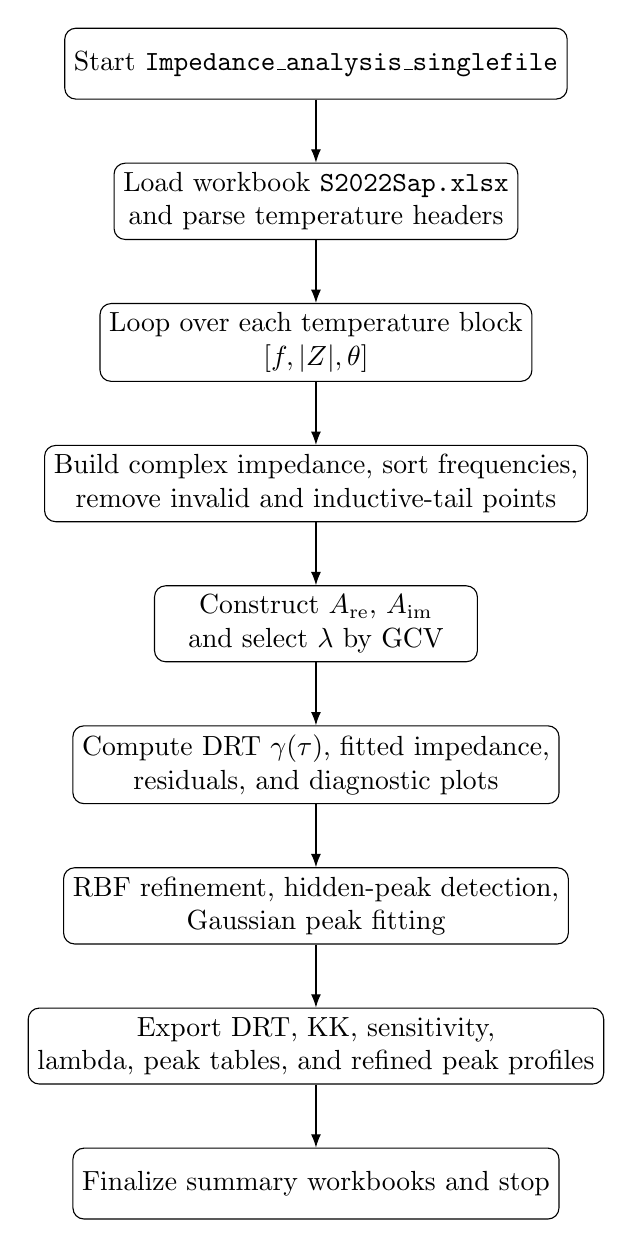
\begin{tikzpicture}[
	node distance=8mm and 10mm,
	block/.style={rectangle, rounded corners, draw, align=center, minimum width=4.1cm, minimum height=9mm},
	decision/.style={diamond, draw, align=center, aspect=2, inner sep=1pt},
	line/.style={-Latex}
]
\node[block] (start) {Start \texttt{Impedance\_analysis\_singlefile}};
\node[block, below=of start] (load) {Load workbook \texttt{S2022Sap.xlsx} \\ and parse temperature headers};
\node[block, below=of load] (split) {Loop over each temperature block \\ $[f, |Z|, \theta]$};
\node[block, below=of split] (pre) {Build complex impedance, sort frequencies, \\ remove invalid and inductive-tail points};
\node[block, below=of pre] (gcv) {Construct $A_{\mathrm{re}}$, $A_{\mathrm{im}}$ \\ and select $\lambda$ by GCV};
\node[block, below=of gcv] (drt) {Compute DRT $\gamma(\tau)$, fitted impedance, \\ residuals, and diagnostic plots};
\node[block, below=of drt] (peaks) {RBF refinement, hidden-peak detection, \\ Gaussian peak fitting};
\node[block, below=of peaks] (exports) {Export DRT, KK, sensitivity, \\ lambda, peak tables, and refined peak profiles};
\node[block, below=of exports] (end) {Finalize summary workbooks and stop};

\draw[line] (start) -- (load);
\draw[line] (load) -- (split);
\draw[line] (split) -- (pre);
\draw[line] (pre) -- (gcv);
\draw[line] (gcv) -- (drt);
\draw[line] (drt) -- (peaks);
\draw[line] (peaks) -- (exports);
\draw[line] (exports) -- (end);
\end{tikzpicture}
\end{center}

\section{How the MATLAB Functions Map to the Mathematics}

The single-file implementation is structured as a top-level orchestration function plus a set of local helper functions.

\subsection*{Input and Preprocessing Helpers}

\begin{itemize}
\item \texttt{load\_input\_dataset\_2011}: reads the numeric workbook block and extracts temperature labels from the first header row.
\item \texttt{load\_f\_Z\_theta\_2011}: converts the three-column workbook slice into a frequency vector and a complex impedance vector.
\item \texttt{remove\_inductive\_effects\_matlab2011}: removes the contiguous high-frequency tail where $\Im(Z) > 0$, which would otherwise distort the DRT inversion.
\end{itemize}

\subsection*{DRT Inversion and Forward Model Helpers}

\begin{itemize}
\item \texttt{calc\_A\_re\_matlab2011} and \texttt{calc\_A\_im\_matlab2011}: assemble the discrete real and imaginary DRT projection matrices.
\item \texttt{TR\_DRT\_matlab2011}: solves the full non-negative Tikhonov-regularized inverse problem.
\item \texttt{tr\_drt\_gcv\_impart\_matlab2011} and \texttt{tr\_drt\_gcv\_repart\_matlab2011}: solve the component-wise ridge problems used during GCV scoring.
\item \texttt{calculate\_EIS\_matlab2011}: performs the forward projection from the recovered DRT back to complex impedance.
\end{itemize}

\subsection*{Peak Refinement Helpers}

\begin{itemize}
\item \texttt{create\_rbf\_model\_2011} and \texttt{rbf\_eval\_2011}: interpolate the raw DRT onto a dense log-time grid.
\item \texttt{detect\_hidden\_peaks\_second\_derivative\_2011}: identifies shoulder-like peaks through curvature analysis.
\item \texttt{fit\_rbf\_gaussian\_peaks\_2011}: fits a Gaussian sum to the refined DRT profile, converts peak area to $R$, center to $\tau$, and then uses the current heuristic formula for $n$.
\item \texttt{build\_refined\_peak\_profile\_export\_2011}: exports the dense RBF curve, summed fit, baseline, and each individual fitted Gaussian component to Excel.
\end{itemize}

\subsection*{Validation and Reporting Helpers}

\begin{itemize}
\item \texttt{perform\_kk\_test\_matlab2011} and \texttt{solve\_kk\_candidate\_matlab2011}: estimate KK-consistent surrogates and summarize residual quality.
\item \texttt{perform\_sensitivity\_analysis\_matlab2011}: bootstrap the selected DRT to obtain uncertainty bands.
\item \texttt{perform\_lambda\_perturbation\_sensitivity\_matlab2011}: quantify how strongly the selected fit depends on local lambda changes.
\item \texttt{write\_matrix\_with\_header\_2011}: writes each per-temperature result sheet to Excel.
\end{itemize}

\section{DRT Representation}

We use the DRT representation
\begin{equation}
Z(\omega) = R_{\infty} + \int_0^{\infty} \frac{\Gamma(\tau)}{1 + i\omega\tau} \, d\ln \tau.
\end{equation}

Equivalently, if we define
\begin{equation}
y = \ln\left(\frac{\tau}{\tau_0}\right),
\qquad
\tau = \tau_0 e^y,
\end{equation}
then
\begin{equation}
Z(\omega) = R_{\infty} + \int_{-\infty}^{\infty} \frac{\gamma(y)}{1 + i\omega\tau_0 e^y} \, dy,
\end{equation}
where
\begin{equation}
\Gamma(\tau) = \gamma\left(\ln\frac{\tau}{\tau_0}\right).
\end{equation}

\section{Discrete Forward Model Used in the MATLAB Code}

The MATLAB workflow discretizes the DRT integral on the measured frequency grid. If the experimental frequencies are
\begin{equation}
f_1, f_2, \dots, f_N,
\qquad
\omega_p = 2\pi f_p,
\end{equation}
and the corresponding relaxation times are approximated by
\begin{equation}
\tau_q \approx \frac{1}{f_q},
\end{equation}
then the real and imaginary parts of the impedance are approximated by matrix-vector products
\begin{align}
\Re(Z) &\approx R_{\infty}\bm{1} + A_{\mathrm{re}}\bm{\gamma}, \\
\Im(Z) &\approx A_{\mathrm{im}}\bm{\gamma}.
\end{align}

Here $\bm{\gamma} \in \mathbb{R}^N$ is the discretized DRT vector and the matrices $A_{\mathrm{re}}$ and $A_{\mathrm{im}}$ are assembled in the MATLAB functions \texttt{calc\_A\_re\_matlab2011} and \texttt{calc\_A\_im\_matlab2011}. Their entries are
\begin{align}
\left(A_{\mathrm{re}}\right)_{pq} &= -\frac{1}{2}\frac{\Delta \ln \tau_q}{1 + (\omega_p \tau_q)^2}, \\
\left(A_{\mathrm{im}}\right)_{pq} &= \frac{1}{2}\frac{\omega_p \tau_q}{1 + (\omega_p \tau_q)^2}\,\Delta \ln \tau_q,
\end{align}
where the code approximates the local log-width by neighboring values,
\begin{equation}
\Delta \ln \tau_q \approx
\begin{cases}
\ln(\tau_{q+1}/\tau_q), & q=1, \\
\ln(\tau_q/\tau_{q-1}), & q=N, \\
\ln(\tau_{q+1}/\tau_{q-1}), & 1<q<N.
\end{cases}
\end{equation}

This converts the continuous DRT inversion into a finite-dimensional constrained inverse problem.

\section{Tikhonov Regularization and Non-Negative DRT Recovery}

The DRT inversion is ill-posed: small perturbations in the impedance data can lead to large oscillations in the recovered DRT. The MATLAB code therefore uses first-level Tikhonov regularization together with a non-negativity constraint.

The full inversion solved by \texttt{TR\_DRT\_matlab2011} is
\begin{equation}
\min_{\bm{\gamma} \ge 0,\, R_{\infty}} 
\left\|
\begin{bmatrix}
A_{\mathrm{re}} & \bm{1} \\
A_{\mathrm{im}} & \bm{0} \\
\sqrt{\lambda/2}\,I & \bm{0}
\end{bmatrix}
\begin{bmatrix}
\bm{\gamma} \\
R_{\infty}
\end{bmatrix}
-
\begin{bmatrix}
\Re(\bm{Z}_{\mathrm{exp}}) \\
\Im(\bm{Z}_{\mathrm{exp}}) \\
\bm{0}
\end{bmatrix}
\right\|_2^2.
\end{equation}

Equivalently, this is the constrained minimization of
\begin{equation}
\|\Re(\bm{Z}_{\mathrm{exp}}) - (R_{\infty}\bm{1} + A_{\mathrm{re}}\bm{\gamma})\|_2^2
+ \|\Im(\bm{Z}_{\mathrm{exp}}) - A_{\mathrm{im}}\bm{\gamma}\|_2^2
+ \frac{\lambda}{2}\|\bm{\gamma}\|_2^2,
\end{equation}
subject to $\bm{\gamma} \ge 0$.

The role of each term is:

\begin{itemize}
\item the first term fits the real part of the measured impedance,
\item the second term fits the imaginary part,
\item the third term penalizes large or oscillatory DRT amplitudes,
\item the non-negativity constraint enforces a physically interpretable relaxation spectrum.
\end{itemize}

Larger $\lambda$ produces smoother spectra with larger residuals, while smaller $\lambda$ produces sharper spectra that risk overfitting measurement noise.

\section{Residuals Used Throughout the Workflow}

Once a candidate DRT $\bm{\gamma}$ and resistance $R_{\infty}$ are found, the code reconstructs the fitted impedance
\begin{equation}
\bm{Z}_{\mathrm{cal}} = R_{\infty}\bm{1} + A_{\mathrm{re}}\bm{\gamma} + iA_{\mathrm{im}}\bm{\gamma}.
\end{equation}

The complex residual vector is
\begin{equation}
\bm{r} = \bm{Z}_{\mathrm{exp}} - \bm{Z}_{\mathrm{cal}}.
\end{equation}

The code reports summary residual metrics such as
\begin{align}
\text{mean absolute residual} &= \frac{1}{N}\sum_{p=1}^N |r_p|, \\
\text{max absolute residual} &= \max_p |r_p|.
\end{align}

These same residuals also drive the lambda perturbation study and the bootstrap sensitivity analysis.

\section{Component-Wise Inversion and Cross-Validation Logic}

The MATLAB code does not choose $\lambda$ from the full Tikhonov solve directly. Instead, it evaluates each candidate $\lambda$ by solving two component-wise problems.

For the imaginary-only branch, the code solves
\begin{equation}
\min_{\bm{\gamma} \ge 0}
\left\|
\begin{bmatrix}
A_{\mathrm{im}} \\
\sqrt{\lambda/2}\,I
\end{bmatrix}
\bm{\gamma}
-
\begin{bmatrix}
\Im(\bm{Z}_{\mathrm{exp}}) \\
\bm{0}
\end{bmatrix}
\right\|_2^2.
\end{equation}

Then $R_{\infty}$ is estimated afterwards by averaging the real-part mismatch:
\begin{equation}
R_{\infty} = \frac{1}{N}\sum_{p=1}^N \left(\Re(Z_{\mathrm{exp},p}) - (A_{\mathrm{re}}\bm{\gamma})_p\right).
\end{equation}

For the real-only branch, the code solves
\begin{equation}
\min_{\bm{\gamma} \ge 0}
\left\|
\begin{bmatrix}
A_{\mathrm{re}} \\
\sqrt{\lambda/2}\,I
\end{bmatrix}
\bm{\gamma}
-
\begin{bmatrix}
\Re(\bm{Z}_{\mathrm{exp}}) \\
\bm{0}
\end{bmatrix}
\right\|_2^2.
\end{equation}

This gives two channel-specific DRT estimates. The workflow then uses both real and imaginary residuals to assess whether the selected $\lambda$ generalizes across components rather than merely fitting one channel in isolation.

\section{Generalized Cross-Validation Criterion}

For each candidate $\lambda$, the code forms the stacked residual norm
\begin{equation}
\mathrm{RSS}(\lambda) = \left\|
\begin{bmatrix}
\Re(\bm{Z}_{\mathrm{exp}}) - (R_{\infty}\bm{1} + A_{\mathrm{re}}\bm{\gamma}) \\
\Im(\bm{Z}_{\mathrm{exp}}) - A_{\mathrm{im}}\bm{\gamma}
\end{bmatrix}
\right\|_2^2.
\end{equation}

Let $N$ be the number of frequencies and $M = 2N$ the total number of real-valued data equations. The code computes a normalized GCV score of the form
\begin{equation}
\mathrm{nGCV}(\lambda) = \frac{\mathrm{RSS}(\lambda)/M}{\left(1 - \mathrm{tr}(H_\lambda)/N\right)^2},
\end{equation}
where $H_\lambda$ is the effective hat matrix of the corresponding ridge problem.

For the imaginary-only branch, the code uses
\begin{equation}
H_\lambda^{(\mathrm{im})} = A_{\mathrm{im}}\left(A_{\mathrm{im}}^T A_{\mathrm{im}} + \frac{\lambda}{2}I\right)^{-1}A_{\mathrm{im}}^T,
\end{equation}
and analogously for the real-only branch,
\begin{equation}
H_\lambda^{(\mathrm{re})} = A_{\mathrm{re}}\left(A_{\mathrm{re}}^T A_{\mathrm{re}} + \frac{\lambda}{2}I\right)^{-1}A_{\mathrm{re}}^T.
\end{equation}

The traces $\mathrm{tr}(H_\lambda)$ are computed in the MATLAB helpers \texttt{hat\_trace\_impart\_matlab2011} and \texttt{hat\_trace\_repart\_matlab2011}. They act as effective degrees of freedom: larger trace means a more flexible fit.

Conceptually, GCV balances two effects:

\begin{itemize}
\item small residual error favors small $\lambda$,
\item low effective complexity favors larger $\lambda$.
\end{itemize}

The denominator penalizes models whose effective degrees of freedom approach the data count.

\section{GCV Slope Criterion and Lambda Selection Policy}

The code computes the discrete log-slope of the GCV curve,
\begin{equation}
\frac{d\ln G}{d\ln \lambda} \approx \frac{\ln G_{i+1} - \ln G_i}{\ln \lambda_{i+1} - \ln \lambda_i},
\end{equation}
where $G_i = \mathrm{nGCV}(\lambda_i)$.

This slope is used to detect a flat region of the GCV curve. In the code, a segment is considered flat when
\begin{equation}
\left|\frac{d\ln G}{d\ln \lambda}\right| \le 0.002.
\end{equation}

If such a flat region exists, the workflow selects the largest $\lambda$ in that flat zone. This policy prefers the smoothest DRT that still lies on the GCV plateau. If no flat region is detected, the code falls back to the minimum-GCV solution:
\begin{equation}
\lambda_{\mathrm{best}} = \arg\min_{\lambda} \mathrm{nGCV}(\lambda).
\end{equation}

Thus the MATLAB selection policy is a hybrid of plateau detection and standard GCV minimization.

\begin{figure}[h]
\centering
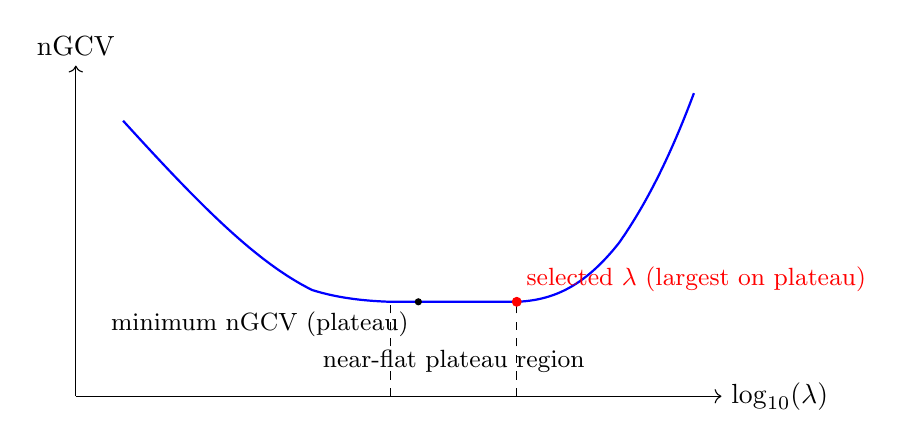
\begin{tikzpicture}[x=1cm,y=1cm]
\draw[->] (0,0) -- (8.2,0) node[right] {$\log_{10}(\lambda)$};
\draw[->] (0,0) -- (0,4.2) node[above] {nGCV};

% Piecewise-like shape with a clear near-horizontal plateau.
\draw[thick,blue] (0.6,3.5) .. controls (1.6,2.4) and (2.3,1.7) .. (3.0,1.35)
				 .. controls (3.35,1.24) and (3.7,1.21) .. (4.0,1.20)
				 -- (5.6,1.20)
				 .. controls (6.05,1.22) and (6.45,1.38) .. (6.9,1.95)
				 .. controls (7.25,2.45) and (7.55,3.05) .. (7.85,3.85);

\draw[dashed] (4.0,0) -- (4.0,1.2);
\draw[dashed] (5.6,0) -- (5.6,1.2);
\node[align=center,font=\small] at (4.8,0.45) {near-flat\ plateau region};

\fill[red] (5.6,1.20) circle (1.8pt);
\node[red,above right,font=\small] at (5.6,1.20) {selected $\lambda$\ (largest on plateau)};

\fill[black] (4.35,1.20) circle (1.3pt);
\node[black,below left,font=\small] at (4.35,1.20) {minimum nGCV (plateau)};
\end{tikzpicture}
\caption{Illustrative nGCV-vs-$\lambda$ profile showing the plateau-based selection policy used in the MATLAB workflow.}
\end{figure}

\section{Lambda Perturbation and Local Residual Sensitivity}

After selecting $\lambda_{\mathrm{ref}}$, the code perturbs it by multiplicative factors
\begin{equation}
0.3,\; 0.5,\; 0.7,\; 1.0,\; 1.5,\; 2.0,\; 3.0
\end{equation}
and recomputes the fit residual at each perturbed value.

If the reference mean residual is $\bar{r}_{\mathrm{ref}}$ and the perturbed mean residual is $\bar{r}(\lambda)$, then the reported percent change is
\begin{equation}
\Delta_{\%}(\lambda) = 100\frac{\bar{r}(\lambda) - \bar{r}_{\mathrm{ref}}}{\max(\bar{r}_{\mathrm{ref}}, \varepsilon)}.
\end{equation}

This is not a second cross-validation criterion. Rather, it is a post-selection robustness diagnostic: if $\Delta_{\%}$ changes sharply near the selected $\lambda$, then the chosen inversion is locally sensitive.

\section{Bootstrap Sensitivity Analysis}

To assess the stability of the recovered DRT, the code constructs synthetic spectra by adding complex Gaussian noise to the measured impedance:
\begin{equation}
\bm{Z}_{\mathrm{boot}} = \bm{Z}_{\mathrm{exp}} + \sigma_{\mathrm{re}}\bm{\eta}_{\mathrm{re}} + i\sigma_{\mathrm{im}}\bm{\eta}_{\mathrm{im}},
\end{equation}
where the noise levels $\sigma_{\mathrm{re}}$ and $\sigma_{\mathrm{im}}$ are estimated from the residual statistics of the selected fit, and $\bm{\eta}_{\mathrm{re}}, \bm{\eta}_{\mathrm{im}}$ are standard normal random vectors.

For each bootstrap replicate, the code recomputes
\begin{equation}
\bm{\gamma}^{(k)} = \mathrm{TR\_DRT}(\bm{Z}_{\mathrm{boot}}^{(k)}, \lambda_{\mathrm{best}}).
\end{equation}

From the ensemble of recovered DRT vectors, it reports pointwise mean, standard deviation, quantile bands, and coefficient of variation,
\begin{equation}
\mathrm{CV}(\tau) = 100\frac{\sigma_{\gamma}(\tau)}{\max(\mu_{\gamma}(\tau), \text{floor})}.
\end{equation}

The script also reports a band-area metric obtained by integrating the width of the bootstrap confidence band over $\ln\tau$.

\begin{figure}[h]
\centering
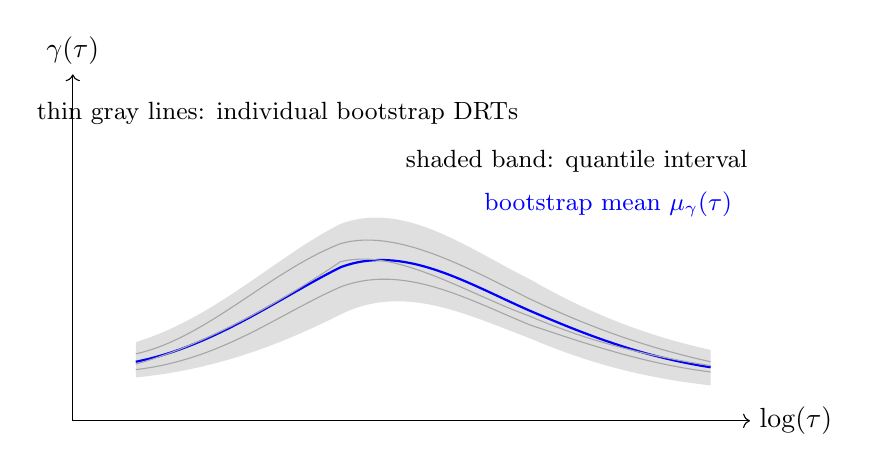
\begin{tikzpicture}[x=1cm,y=1cm]
\draw[->] (0,0) -- (8.6,0) node[right] {$\log(\tau)$};
\draw[->] (0,0) -- (0,4.4) node[above] {$\gamma(\tau)$};

% Uncertainty band (95% region, schematic)
\fill[gray!25] (0.8,1.0) .. controls (1.8,1.3) and (2.6,2.1) .. (3.4,2.5)
			   .. controls (4.2,2.8) and (5.0,2.2) .. (5.8,1.8)
			   .. controls (6.5,1.4) and (7.2,1.1) .. (8.1,0.9)
			   -- (8.1,0.45)
			   .. controls (7.2,0.55) and (6.5,0.75) .. (5.8,1.05)
			   .. controls (5.0,1.35) and (4.2,1.75) .. (3.4,1.35)
			   .. controls (2.6,0.95) and (1.8,0.65) .. (0.8,0.55) -- cycle;

% Mean curve
\draw[thick,blue] (0.8,0.75) .. controls (1.8,0.95) and (2.6,1.55) .. (3.4,1.95)
				 .. controls (4.2,2.25) and (5.0,1.75) .. (5.8,1.4)
				 .. controls (6.5,1.1) and (7.2,0.82) .. (8.1,0.68);

% A few bootstrap sample curves
\draw[thin,gray!70] (0.8,0.85) .. controls (1.7,1.05) and (2.5,1.9) .. (3.4,2.25)
				   .. controls (4.1,2.45) and (5.0,1.95) .. (5.8,1.55)
				   .. controls (6.5,1.22) and (7.2,0.95) .. (8.1,0.75);
\draw[thin,gray!70] (0.8,0.65) .. controls (1.9,0.78) and (2.6,1.35) .. (3.4,1.7)
				   .. controls (4.2,2.0) and (5.0,1.55) .. (5.8,1.22)
				   .. controls (6.6,0.95) and (7.3,0.72) .. (8.1,0.62);
\draw[thin,gray!70] (0.8,0.72) .. controls (1.8,1.0) and (2.8,1.62) .. (3.4,2.02)
				   .. controls (4.1,2.2) and (5.0,1.62) .. (5.8,1.33)
				   .. controls (6.5,1.03) and (7.2,0.84) .. (8.1,0.7);

\node[font=\small,blue] at (6.8,2.75) {bootstrap mean $\mu_\gamma(\tau)$};
\node[font=\small] at (6.4,3.3) {shaded band: quantile interval};
\node[font=\small] at (2.6,3.9) {thin gray lines: individual bootstrap DRTs};
\end{tikzpicture}
\caption{Illustrative bootstrap-sensitivity view: individual bootstrap DRT reconstructions, mean curve, and uncertainty band over $\log(\tau)$.}
\end{figure}

\section{Kramers-Kronig Consistency Test Used in the Code}

The KK test in the MATLAB file fits the impedance with a finite set of Debye-like branches plus series resistance and inductance. For a candidate basis size $n_b$ and regularization weight $\alpha$, the model is
\begin{equation}
Z_{\mathrm{KK}}(\omega) = R_{\infty} + \sum_{j=1}^{n_b} \frac{R_j}{1 + i\omega\tau_j} + i\omega L.
\end{equation}

In real and imaginary parts this is represented by matrices $B_{\mathrm{re}}$ and $B_{\mathrm{im}}$ whose entries are
\begin{align}
\left(B_{\mathrm{re}}\right)_{pj} &= \frac{1}{1 + (\omega_p \tau_j)^2}, \\
\left(B_{\mathrm{im}}\right)_{pj} &= -\frac{\omega_p \tau_j}{1 + (\omega_p \tau_j)^2}.
\end{align}

The constrained least-squares problem solved by the code is
\begin{equation}
\min_{\bm{R} \ge 0,\, R_{\infty},\, L}
\left\|
\begin{bmatrix}
B_{\mathrm{re}} & \bm{1} & \bm{0} \\
B_{\mathrm{im}} & \bm{0} & \bm{\omega} \\
\sqrt{\alpha}I & \bm{0} & \bm{0}
\end{bmatrix}
\begin{bmatrix}
\bm{R} \\
R_{\infty} \\
L
\end{bmatrix}
-
\begin{bmatrix}
\Re(\bm{Z}_{\mathrm{exp}}) \\
\Im(\bm{Z}_{\mathrm{exp}}) \\
\bm{0}
\end{bmatrix}
\right\|_2^2.
\end{equation}

The code tests several candidate basis sizes and regularization values, retains the best solution by total residual percentage, and reports
\begin{align}
\text{real residual \%} &= 100\frac{\|\Re(\bm{r})\|_2}{\|\Re(\bm{Z}_{\mathrm{exp}})\|_2}, \\
\text{imag residual \%} &= 100\frac{\|\Im(\bm{r})\|_2}{\|\Im(\bm{Z}_{\mathrm{exp}})\|_2}, \\
\text{total residual \%} &= 100\frac{\|[\Re(\bm{r});\Im(\bm{r})]\|_2}{\|[\Re(\bm{Z}_{\mathrm{exp}});\Im(\bm{Z}_{\mathrm{exp}})]\|_2}.
\end{align}

The same KK procedure is applied both to the measured impedance and to the DRT-reconstructed impedance as a consistency check on the inversion.

\section{ZARC Element}

A ZARC element may be written as a resistor $R$ in parallel with a constant-phase element (CPE):
\begin{equation}
Y_{\mathrm{CPE}} = Q (i\omega)^n,
\qquad 0 < n \le 1.
\end{equation}

The total admittance is
\begin{equation}
Y(\omega) = \frac{1}{R} + Q(i\omega)^n,
\end{equation}
so the impedance is
\begin{align}
Z(\omega)
&= \frac{1}{Y(\omega)} \\
&= \frac{R}{1 + RQ(i\omega)^n}.
\end{align}

Defining the characteristic time
\begin{equation}
\tau_0 = (RQ)^{1/n},
\end{equation}
the ZARC becomes
\begin{equation}
Z_{\mathrm{ZARC}}(\omega) = \frac{R}{1 + (i\omega\tau_0)^n}.
\end{equation}

In the MATLAB reconstruction used in the workflow, each refined arc is written as
\begin{equation}
Z_k(\omega) = \frac{R_k}{1 + (i\omega R_k C_k)^{n_k}},
\end{equation}
which identifies an effective RC-style time constant
\begin{equation}
\tau_k = R_k C_k.
\end{equation}

\section{Exact DRT of a ZARC}

We seek a DRT density that reproduces
\begin{equation}
Z(\omega) = \frac{R}{1 + (i\omega\tau_0)^n}.
\end{equation}

Define the analytic continuation
\begin{equation}
F(s) = \frac{R}{1 + (s\tau_0)^n}, \qquad \Re(s) > 0.
\end{equation}

The DRT density follows from the Stieltjes inversion formula
\begin{equation}
\Gamma(\tau) = -\frac{1}{\pi} \, \Im\left[F\left(-\frac{1}{\tau} + i0\right)\right].
\end{equation}

Set
\begin{equation}
u = \left(\frac{\tau_0}{\tau}\right)^n.
\end{equation}

On the negative real axis, using the principal branch,
\begin{equation}
\left(-\frac{\tau_0}{\tau} + i0\right)^n = u e^{i\pi n}.
\end{equation}

Therefore,
\begin{equation}
F\left(-\frac{1}{\tau} + i0\right) = \frac{R}{1 + u e^{i\pi n}} = \frac{R}{1 + u\cos(\pi n) + i u\sin(\pi n)}.
\end{equation}

Taking the imaginary part gives
\begin{equation}
\Im(F) = -\frac{R u \sin(\pi n)}{1 + 2u\cos(\pi n) + u^2}.
\end{equation}

Hence the exact DRT is
\begin{equation}
\Gamma(\tau) = \frac{R}{\pi}
\frac{\left(\tau_0/\tau\right)^n \sin(\pi n)}{1 + 2\left(\tau_0/\tau\right)^n \cos(\pi n) + \left(\tau_0/\tau\right)^{2n}}.
\end{equation}

Using $y = \ln(\tau/\tau_0)$, so that $u = e^{-ny}$, this becomes the symmetric log-time form
\begin{equation}
\gamma(y) = \frac{R\sin(\pi n)}{2\pi\left[\cosh(ny) + \cos(\pi n)\right]}.
\end{equation}

This is the exact DRT of a ZARC element.

\section{Derivation: ZARC as an Infinite Series of ZAP Elements}

In this note, define one elementary ZAP element as a single Debye-type relaxation contribution in series,
\begin{equation}
Z_{\mathrm{ZAP}}(\omega;\tau,\Delta R) = \frac{\Delta R}{1+i\omega\tau},
\end{equation}
where $\Delta R>0$ is the resistance weight carried by that relaxation time.

The DRT representation of a passive spectrum is
\begin{equation}
Z(\omega) = R_{\infty} + \int_0^{\infty}\frac{\Gamma(\tau)}{1+i\omega\tau}\,d\ln\tau.
\end{equation}

Now partition the $\ln\tau$ axis into bins with centers $\tau_k$ and widths $\Delta\ln\tau_k$. Then
\begin{equation}
Z(\omega)-R_{\infty}
\approx \sum_{k=1}^{K}\frac{\Gamma(\tau_k)\,\Delta\ln\tau_k}{1+i\omega\tau_k}
=\sum_{k=1}^{K}\frac{\Delta R_k}{1+i\omega\tau_k},
\end{equation}
with
\begin{equation}
\Delta R_k := \Gamma(\tau_k)\,\Delta\ln\tau_k.
\end{equation}

Each summand is exactly one ZAP element in series. Taking the refinement limit $\max_k\Delta\ln\tau_k\to 0$ gives
\begin{equation}
Z(\omega)-R_{\infty}
=\lim_{K\to\infty}\sum_{k=1}^{K}\frac{\Delta R_k}{1+i\omega\tau_k},
\end{equation}
which proves that any DRT-representable impedance is the limit of an infinite series of ZAP elements.

\begin{figure}[h]
\centering
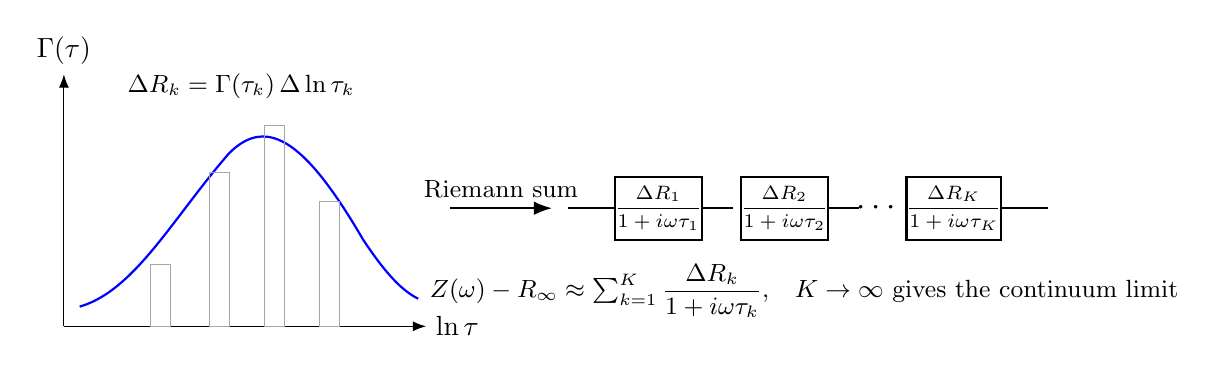
\begin{tikzpicture}[x=1cm,y=1cm,>=Latex]
% Left: continuum density over log tau
\draw[->] (0,0) -- (4.6,0) node[right] {$\ln\tau$};
\draw[->] (0,0) -- (0,3.2) node[above] {$\Gamma(\tau)$};
\draw[thick,blue] (0.2,0.25) .. controls (0.9,0.45) and (1.4,1.4) .. (2.1,2.2)
				 .. controls (2.6,2.7) and (3.1,2.3) .. (3.8,1.1)
				 .. controls (4.1,0.65) and (4.3,0.45) .. (4.5,0.35);

% Bin rectangles to indicate DeltaRk
\draw[gray!70] (1.1,0) rectangle (1.35,0.78);
\draw[gray!70] (1.85,0) rectangle (2.1,1.95);
\draw[gray!70] (2.55,0) rectangle (2.8,2.55);
\draw[gray!70] (3.25,0) rectangle (3.5,1.58);
\node[font=\small,align=center] at (2.25,3.05) {$\Delta R_k=\Gamma(\tau_k)\,\Delta\ln\tau_k$};

% Arrow to right panel
\draw[->,thick] (4.9,1.5) -- (6.2,1.5) node[midway,above,font=\small] {Riemann sum};

% Right: finite/infinite ZAP series
\draw[thick] (6.4,1.5) -- (7.0,1.5);
\draw[thick] (7.0,1.9) rectangle (8.1,1.1);
\node[font=\scriptsize] at (7.55,1.5) {$\dfrac{\Delta R_1}{1+i\omega\tau_1}$};
\draw[thick] (8.1,1.5) -- (8.5,1.5);

\draw[thick] (8.6,1.9) rectangle (9.7,1.1);
\node[font=\scriptsize] at (9.15,1.5) {$\dfrac{\Delta R_2}{1+i\omega\tau_2}$};
\draw[thick] (9.7,1.5) -- (10.1,1.5);

\node[font=\large] at (10.35,1.5) {$\cdots$};

\draw[thick] (10.7,1.9) rectangle (11.9,1.1);
\node[font=\scriptsize] at (11.3,1.5) {$\dfrac{\Delta R_K}{1+i\omega\tau_K}$};
\draw[thick] (11.9,1.5) -- (12.5,1.5);

\node[font=\small,align=center] at (9.4,0.45)
{$Z(\omega)-R_\infty\approx\sum_{k=1}^{K}\dfrac{\Delta R_k}{1+i\omega\tau_k}$,\quad
 $K\to\infty$ gives the continuum limit};
\end{tikzpicture}
\caption{ZARC as a continuum sum of ZAP elements: binning the DRT density over $\ln\tau$ yields a finite Debye/ZAP series, whose refinement limit gives the exact integral representation.}
\end{figure}

For a ZARC specifically,
\begin{equation}
Z_{\mathrm{ZARC}}(\omega)=\frac{R}{1+(i\omega\tau_0)^n},
\end{equation}
and its associated DRT density is
\begin{equation}
\Gamma(\tau) = \frac{R}{\pi}
\frac{\left(\tau_0/\tau\right)^n \sin(\pi n)}{1 + 2\left(\tau_0/\tau\right)^n \cos(\pi n) + \left(\tau_0/\tau\right)^{2n}}.
\end{equation}

Substituting this density into the integral above gives an exact continuum superposition of Debye/ZAP terms with weight
\begin{equation}
dR(\tau)=\Gamma(\tau)\,d\ln\tau,
\end{equation}
and total distributed resistance
\begin{equation}
\int_0^{\infty}\Gamma(\tau)\,d\ln\tau=R.
\end{equation}

So, in the precise mathematical sense used by DRT, one ZARC element is equivalent to an infinite series (continuum sum) of ZAP elements over relaxation time.

\section{Area Under the Peak and Resistance}

In DRT, the resistance contribution of a relaxation process is the area under the peak with respect to $d\ln\tau$:
\begin{equation}
R = \int_{-\infty}^{\infty} \gamma(y) \, dy.
\end{equation}

In the workflow, each refined peak is approximated locally by a Gaussian in log-time,
\begin{equation}
\gamma_{\mathrm{fit}}(y) = A \exp\left[-\frac{(y-\mu)^2}{2\sigma^2}\right].
\end{equation}

The area under this Gaussian is
\begin{equation}
\int_{-\infty}^{\infty} A \exp\left[-\frac{(y-\mu)^2}{2\sigma^2}\right] dy = A\sigma\sqrt{2\pi}.
\end{equation}

This gives the resistance estimate used in the code:
\begin{equation}
R_{\mathrm{est}} = A\sigma\sqrt{2\pi}.
\end{equation}

\section{Peak Detection, RBF Refinement, and Gaussian Peak Model}

The peak-analysis stage is not performed on the raw DRT vector directly. Instead, the code first interpolates the recovered DRT over a dense log-time grid using a Gaussian radial basis function model,
\begin{equation}
\gamma_{\mathrm{RBF}}(x) = \sum_{j=1}^{N} w_j \exp\!\left[-(\varepsilon(x-x_j))^2\right],
\end{equation}
where $x = \ln\tau$.

The base peaks are then detected by local-maxima rules with a minimum height threshold and a minimum separation in sample index. Hidden or shoulder peaks are identified by analyzing the smoothed negative second derivative of the RBF curve. In other words, the code uses curvature maxima in
\begin{equation}
-\frac{d^2\gamma_{\mathrm{RBF}}}{dx^2}
\end{equation}
to locate shoulders that may not appear as strong raw maxima.

After combining base peaks and hidden peaks, the code fits a global Gaussian sum with baseline,
\begin{equation}
\gamma_{\mathrm{fit}}(x) = \sum_{k=1}^{m} A_k \exp\left[-\frac{(x-\mu_k)^2}{2\sigma_k^2}\right] + b,
\end{equation}
where the centers $\mu_k$ are inherited from the refined peak-detection step and the amplitudes, widths, and baseline are optimized numerically.

The objective minimized in the code is a penalized least-squares function,
\begin{equation}
\mathrm{SSE} = \sum_{j}(\gamma_{\mathrm{fit}}(x_j) - \gamma_{\mathrm{RBF}}(x_j))^2 + \text{width penalties} + \text{small-amplitude penalties}.
\end{equation}

This keeps the fitted Gaussian components compact and suppresses numerically unstable peak widths.

\begin{figure}[h]
\centering
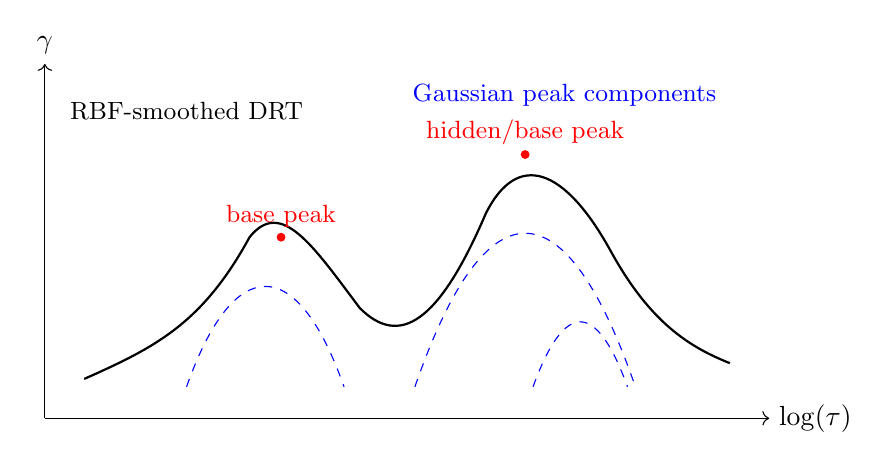
\begin{tikzpicture}[x=1cm,y=1cm]
\draw[->] (0,0) -- (9.2,0) node[right] {$\log(\tau)$};
\draw[->] (0,0) -- (0,4.5) node[above] {$\gamma$};

% raw / rbf-like profile
\draw[thick,black] (0.5,0.5) .. controls (1.4,0.9) and (2.0,1.2) .. (2.6,2.3)
				  .. controls (3.0,2.8) and (3.4,2.2) .. (4.0,1.4)
				  .. controls (4.5,0.9) and (5.0,1.2) .. (5.6,2.6)
				  .. controls (6.0,3.4) and (6.6,3.2) .. (7.2,2.1)
				  .. controls (7.7,1.2) and (8.2,0.9) .. (8.7,0.7);
\node[font=\small] at (1.8,3.9) {RBF-smoothed DRT};

% Gaussian components
\draw[dashed,blue] (1.8,0.4) .. controls (2.4,2.1) and (3.2,2.1) .. (3.8,0.4);
\draw[dashed,blue] (4.7,0.4) .. controls (5.6,3.0) and (6.6,3.0) .. (7.5,0.4);
\draw[dashed,blue] (6.2,0.4) .. controls (6.6,1.5) and (7.0,1.5) .. (7.4,0.4);
\node[blue,font=\small] at (6.6,4.1) {Gaussian peak components};

\fill[red] (3.0,2.3) circle (1.6pt);
\fill[red] (6.1,3.35) circle (1.6pt);
\node[red,font=\small,above] at (3.0,2.3) {base peak};
\node[red,font=\small,above] at (6.1,3.35) {hidden/base peak};
\end{tikzpicture}
\caption{Illustrative peak-refinement stage: RBF-smoothed DRT profile and Gaussian component decomposition used to export per-peak parameters.}
\end{figure}

\section{Time Constant and Capacitance-Style Parameter}

The fitted center gives the peak relaxation time:
\begin{equation}
\tau_{\mathrm{peak}} = e^{\mu}.
\end{equation}

The workflow then forms an effective capacitance-style quantity from
\begin{equation}
\tau_{\mathrm{peak}} = R_{\mathrm{est}} C_{\mathrm{est}},
\end{equation}
so that
\begin{equation}
C_{\mathrm{est}} = \frac{\tau_{\mathrm{peak}}}{R_{\mathrm{est}}}.
\end{equation}

For a true ZARC, the parallel element is a CPE with parameter $Q$, so $C_{\mathrm{est}}$ should be read as an effective RC-style summary rather than an exact ideal capacitance whenever $n < 1$.

\section{Heuristic Calculation of $R$, $C$, and $n$ in the Present MATLAB Workflow}

For each Gaussian component recovered from the refined peak fit, the code exports the following quantities:

\begin{align}
R_k &= A_k \sigma_k \sqrt{2\pi}, \\
\tau_k &= e^{\mu_k}, \\
C_k &= \frac{\tau_k}{R_k}, \\
n_k &= \frac{1.144}{1 + \sigma_k}.
\end{align}

The first three relations follow naturally from the Gaussian approximation to the DRT peak: area gives resistance, the center gives relaxation time, and $\tau = RC$ supplies an effective capacitance. The final relation for $n$ is heuristic in the present code. It enforces the trend that broader peaks imply lower $n$, but it is not derived from the Tikhonov inversion itself.

\section{FWHM-Based $n$ Formula and Check of the $1.144/n$ Expression}

From the exact ZARC DRT profile, the width relation is
\begin{equation}
\mathrm{FWHM}_{\mathrm{Gauss}} = 2\sqrt{2\ln 2}\,\sigma,
\qquad
\mathrm{FWHM}_{\mathrm{ZARC}}(n) = \frac{2}{n}\operatorname{arcosh}\left(2+\cos(\pi n)\right),
\end{equation}
and the theory-based $n$ is defined implicitly by
\begin{equation}
\mathrm{FWHM}_{\mathrm{ZARC}}(n) = \mathrm{FWHM}_{\mathrm{Gauss}}.
\end{equation}

So the mathematically correct FWHM-based statement is an implicit equation in $n$, solved numerically; it is \emph{not} a direct closed form like $n = 1.144/\sigma$ or $n = 1.144/n$.

For the current MATLAB heuristic,
\begin{equation}
n = \frac{1.144}{1+\sigma},
\end{equation}
the exact rearrangement is
\begin{equation}
\sigma = \frac{1.144}{n} - 1.
\end{equation}

Therefore, if one writes only ``$1.144/n$'', that is incomplete for this heuristic mapping. The correct relation needs the minus one term.

As an additional approximation tied to the ZARC-width derivation near $n\approx 1$, one commonly gets a rational form
\begin{equation}
n \approx \frac{a}{a+\sigma},
\qquad a \approx \frac{\pi}{\sqrt{2}} \approx 2.221,
\end{equation}
which has the same qualitative trend as the heuristic but with a theory-derived scale constant.

\section{Exact FWHM of the ZARC DRT}

The peak maximum occurs at $y=0$:
\begin{equation}
\gamma(0) = \frac{R\sin(\pi n)}{2\pi[1 + \cos(\pi n)]}.
\end{equation}

Define the normalized peak shape
\begin{equation}
f(y) = \frac{\gamma(y)}{\gamma(0)} = \frac{1 + \cos(\pi n)}{\cosh(ny) + \cos(\pi n)}.
\end{equation}

The half-maximum condition is
\begin{equation}
f(y_{1/2}) = \frac{1}{2}.
\end{equation}

Therefore,
\begin{align}
\frac{1 + \cos(\pi n)}{\cosh(ny_{1/2}) + \cos(\pi n)} &= \frac{1}{2}, \\
2[1 + \cos(\pi n)] &= \cosh(ny_{1/2}) + \cos(\pi n), \\
\cosh(ny_{1/2}) &= 2 + \cos(\pi n).
\end{align}

Thus,
\begin{equation}
y_{1/2} = \frac{1}{n} \operatorname{arcosh}\left(2 + \cos(\pi n)\right),
\end{equation}
and the exact full width at half maximum in log-time is
\begin{equation}
\boxed{\mathrm{FWHM}_{\mathrm{ZARC}}(n) = \frac{2}{n} \operatorname{arcosh}\left(2 + \cos(\pi n)\right)}.
\end{equation}

\section{FWHM of the Gaussian Peak Fit}

For a Gaussian
\begin{equation}
g(y) = A \exp\left[-\frac{(y-\mu)^2}{2\sigma^2}\right],
\end{equation}
the full width at half maximum is
\begin{equation}
\boxed{\mathrm{FWHM}_{\mathrm{Gauss}} = 2\sqrt{2\ln 2}\,\sigma}.
\end{equation}

\section{Theory-Based Estimate of $n$ from the Fitted Peak Width}

To map the refined Gaussian width to a ZARC exponent from theory, one may equate the Gaussian FWHM to the exact ZARC DRT FWHM:
\begin{equation}
2\sqrt{2\ln 2}\,\sigma = \frac{2}{n} \operatorname{arcosh}\left(2 + \cos(\pi n)\right).
\end{equation}

Equivalently,
\begin{equation}
\sqrt{2\ln 2}\,\sigma = \frac{1}{n} \operatorname{arcosh}\left(2 + \cos(\pi n)\right).
\end{equation}

This relation is implicit in $n$. There is no simple closed-form algebraic inverse, so a theory-based $n$ can be computed numerically by solving
\begin{equation}
g(n) = \frac{2}{n} \operatorname{arcosh}\left(2 + \cos(\pi n)\right) - 2\sqrt{2\ln 2}\,\sigma = 0
\end{equation}
for $0 < n \le 1$.

\section{Current Code Formula for $n$}

The current single-file MATLAB workflow keeps the heuristic form
\begin{equation}
n \approx \frac{1.144}{1 + \sigma}
\end{equation}
for the exported peak parameter $n$. This form is not derived from the exact ZARC DRT above. It only imposes the qualitative trend that broader DRT peaks should correspond to smaller $n$.

The FWHM-based relation derived in this note is theory-linked because it comes directly from the exact DRT shape of the ZARC element, but it is presented here as a derivation and alternative mapping, not as the active formula in the present single-file code.

\section{Summary of Formulas}

For each refined peak:
\begin{align}
R_{\mathrm{est}} &= A\sigma\sqrt{2\pi}, \\
\tau_{\mathrm{peak}} &= e^{\mu}, \\
C_{\mathrm{est}} &= \frac{\tau_{\mathrm{peak}}}{R_{\mathrm{est}}}, \\
\mathrm{FWHM}_{\mathrm{Gauss}} &= 2\sqrt{2\ln 2}\,\sigma, \\
\mathrm{FWHM}_{\mathrm{ZARC}}(n) &= \frac{2}{n} \operatorname{arcosh}\left(2 + \cos(\pi n)\right), \\
n_{\mathrm{heuristic}} &= \frac{1.144}{1 + \sigma}.
\end{align}

If one wants a theory-based alternative, then $n_{\mathrm{est}}$ may instead be defined implicitly by
\begin{equation}
\mathrm{FWHM}_{\mathrm{ZARC}}(n_{\mathrm{est}}) = \mathrm{FWHM}_{\mathrm{Gauss}}.
\end{equation}

Thus the present code uses the heuristic $n_{\mathrm{heuristic}}$, while the FWHM-based relation in this note gives the derivation-based alternative.

\section{Code Output Inventory}

For each input workbook, the MATLAB script writes multiple Excel workbooks keyed by a filesystem-safe sample tag:

\begin{itemize}
\item \texttt{\_analysis\_result.xlsx}: the raw DRT vectors per temperature,
\item \texttt{\_peak\_result.xlsx}: the legacy compact peak matrix,
\item \texttt{\_peak\_detail\_result.xlsx}: the refined per-peak $\tau$, amplitude, $\sigma$, FWHM, $R$, $C$, and $n$ table,
\item \texttt{\_temperature\_plot\_data.xlsx}: Nyquist, DRT, KK, and peak-marker tables for plotting,
\item \texttt{\_refined\_peak\_profiles.xlsx}: dense per-temperature refined peak curves for post-processing,
\item \texttt{\_kk\_result.xlsx}, \texttt{\_sensitivity\_result.xlsx}, and \texttt{\_lambda\_perturbation\_result.xlsx}: diagnostic outputs.
\end{itemize}

The refined peak profile workbook is especially important when individual Gaussian peak components need to be analyzed temperature-by-temperature outside MATLAB.

\section{Detailed RBF Interpolation and Gaussian Basis Fitting Theory}

\subsection{Radial Basis Function Model}

The first refinement step constructs a smooth continuous model of the DRT using Gaussian radial basis functions (RBF). Given discrete DRT points $\{x_j, y_j\}$ where $x_j = \ln(\tau_j)$ and $y_j = \gamma(\tau_j)$, the RBF model is
\begin{equation}
\gamma_{\mathrm{RBF}}(x) = \sum_{j=1}^{N} w_j \exp\!\left[-(\varepsilon \cdot d_j)^2\right],
\end{equation}
where $d_j = |x - x_j|$ is the Euclidean distance and $\varepsilon$ is a shape parameter that determines the width of each Gaussian basis.

The shape parameter is computed from the data spacing as
\begin{equation}
\varepsilon = \frac{1}{\Delta x_{\mathrm{med}}},
\end{equation}
where $\Delta x_{\mathrm{med}}$ is the median spacing between sorted training points $x_j$.

The weights $w_j$ are obtained by solving the regularized least-squares system,
\begin{equation}
\left(\mathbf{\Phi} + \lambda_{\mathrm{RBF}} \mathbf{I}\right) \mathbf{w} = \mathbf{y},
\end{equation}
where $\mathbf{\Phi}$ is the Gaussian kernel matrix with entries $\Phi_{ij} = \exp[-({\varepsilon d_{ij}})^2]$, $\lambda_{\mathrm{RBF}} = 10^{-8}$ is a small Tikhonov regularization parameter for numerical stability, and $\mathbf{y}$ is the vector of DRT values.

\subsection{Base Peak Detection}

Base peaks are identified by simple local-maxima detection on the RBF-interpolated curve. A point $i$ is marked as a local maximum if
\begin{equation}
\gamma_{\mathrm{RBF}}(x_i) \geq \gamma_{\mathrm{RBF}}(x_{i-1}) \quad \text{and} \quad \gamma_{\mathrm{RBF}}(x_i) > \gamma_{\mathrm{RBF}}(x_{i+1}),
\end{equation}
with a minimum height threshold
\begin{equation}
\gamma_{\mathrm{RBF}}(x_i) \geq h_{\min} = 0.05 \cdot \max_j \gamma_{\mathrm{RBF}}(x_j).
\end{equation}

Peaks are then sorted by height in descending order and culled to enforce minimum separation: if two peaks are within $\Delta x_{\mathrm{sep}} = 20$ sample indices, only the taller peak is retained.

\subsection{Hidden Peak Detection via Second Derivative}

Hidden or shoulder peaks are identified by analyzing the smoothed negative second derivative (curvature) of the RBF curve. The curvature signal is defined as
\begin{equation}
\kappa(x_i) = \max\left(0, -\frac{d^2\gamma_{\mathrm{RBF}}}{dx^2}\right),
\end{equation}
capturing regions of concavity. This signal is smoothed using a Savitzky-Golay filter (frame length 7, polynomial order 2).

Peaks in the curvature signal are detected with a threshold
\begin{equation}
\kappa_{\min} = \max\left(0.3 \cdot \max_j \kappa(x_j), 3.2 \cdot \sigma_{\kappa}\right),
\end{equation}
where $\sigma_{\kappa}$ is the standard deviation of $\kappa(x)$.

Each curvature peak passes multi-stage filters: proximity to base peaks, minimum amplitude, local floor, prominence, and interior checks. The final set is capped at $\lfloor m_b / 2 \rfloor$ to prevent over-segmentation.

\subsection{Gaussian Sum Fitting}

The code fits a parametric Gaussian sum plus baseline:
\begin{equation}
\gamma_{\mathrm{fit}}(x) = \sum_{k=1}^{m} A_k \exp\left[-\frac{(x - \mu_k)^2}{2\sigma_k^2}\right] + b,
\end{equation}
where centers $\mu_k$ are fixed at detected peak locations and amplitudes, widths, and baseline are optimized.

The penalized least-squares objective is
\begin{equation}
\mathcal{J}(\mathbf{A}, \boldsymbol{\sigma}, b) = \sum_{j} \left[\gamma_{\mathrm{fit}}(x_j) - \gamma_{\mathrm{RBF}}(x_j)\right]^2 
+ 10^3 \cdot P_\sigma(\boldsymbol{\sigma}) + 10^{-2} \cdot P_A(\mathbf{A}),
\end{equation}
with width penalty enforcing $\sigma_k \in [0.04, 0.90]$ and amplitude penalty enforcing positivity. Optimization uses the simplex method, and given optimal widths, amplitudes are obtained by non-negative least squares.

\subsection{Per-Peak Circuit Parameter Extraction}

\subsubsection{Resistance from Peak Area}

The resistance is the integral of the DRT:
\begin{equation}
R_k = A_k \sigma_k \sqrt{2\pi}.
\end{equation}

\subsubsection{Characteristic Time and Capacitance}

The characteristic relaxation time is the peak center:
\begin{equation}
\tau_k = \exp(\mu_k), \quad C_k = \frac{\tau_k}{R_k}.
\end{equation}

\subsubsection{CPE Exponent Estimation}

The \textbf{empirically optimal} formula (tested on S2022 data, 2.99\% lower Nyquist residuals) is the heuristic:
\begin{equation}
n_k = \frac{1.144}{1 + \sigma_k}.
\end{equation}

Alternative formulas for comparison:

\textbf{FWHM-based implicit formula:} Solving numerically from
\begin{equation}
\sqrt{2\ln 2} \cdot \sigma_k \cdot n_k = \operatorname{acosh}(2 + \cos(\pi n_k)).
\end{equation}

\textbf{Phase-angle method:}
\begin{equation}
n_k = -\frac{4\phi_{\text{apex}}}{\pi},
\end{equation}
where $\phi_{\text{apex}} = -\pi n / 4$ is the phase angle at peak impedance.


\end{document}